%! TEX root = ../main.tex 

\chapter{The Pierre Auger Observatory}
\label{chap:pierre-auger-observatory}

The \PAO is the largest scientific experiment in the world, spanning an area of
roughly \SI{3000}{\kilo\meter\squared}. It consists of an array of 1660 \WCDs, 
which form the \SD, and 27 fluorescence telescopes, that comprise the \FD. The
simultaneous detection of \CR-artifacts in the air and on ground via this hybrid
approach offers a unique possibility to observe \UHECRs at the tail-end of the 
\CR energy spectrum.

%We begin this chapter in \cref{sec:science-case} by formulating open questions 
%that the \PAO aims to answer. Design details for the \FD and for the \SD are 
%given in \cref{sec:fd} and \cref{sec:sd} respectively. After a discussion of the
%local \DAQ processes and the centralized event detection in \cref{sec:cdas}, we 
%finish by detailing the procedure of the event reconstruction and higher level 
%analysis in \cref{sec:rec}.

\section{Project History and Science Goal}
\label{sec:science-case}

The project that is today known as the \acl{PAO} looks back on a history which 
spans more than three decades in total. First plans for a \CR detector of
immense exposure were devised by Nobel laureate James Cronin 
\cite{nobelprizeoutreach2025NobelPrizePhysics} and Faraday medalist Alan Watson 
\cite{FellowWinsIoP2011} at the 22nd \ICRC \cite{watsonDevelopmentPierreAuger}.
They realized that the flux of \UHECRs is very low 
($\approx\SI{6}{\per\km\squared\per\year}$ for energies above \SI{5e18}{\eV}) 
\cite{fenuCosmicRayEnergy2023}), and that one needs to observe a large area over
a long timespan to make statistically relevant statements about their dynamics.

Cronin and Watson gathered support for their ideas and, in 1995, founded a 
collaboration of 140 likeminded scientists in 17 participating countries. A 
white paper was published that outlined the design, capabilities, and cost of 
the \PAO \cite{theaugercollaborationPierreAugerObservatory}. The detector
configuration in use today varies from the concepts presented in this document.
Most importantly, what was originally envisioned by Cronin to be a detector with
an active area of \SI{5000}{\km\squared} spread over two locations (Auger North 
and Auger South) had to be amended and only one site with and area of 
\SI{3000}{\km\squared}, located in the Argentinian Pampa Amarilla in the Mendoza
province, could be realized. There, construction of an Engineering Array - a 
full scale prototype of the first \SD and \FD detectors (see \cref{sec:sd} and 
\cref{sec:fd} respectively) was completed in 2001. More hardware was added after
initial tests, making the \PAO the largest observatory for \CRs by the end of 
2003.

Since this time, the observatory has made fundamental contributions to several 
important sub-fields of astroparticle physics. 

Science results
Open Data
AugerPrime review
Decomissioning? (Antonellas mail)


\cite{abraham_properties_2004} and will continue to yield results until 
decomission after 2030 \cite{castellina_outcome_2023}.

Many insights, such as the existence of the \CR dipole discussed in
\cref{sec:cr-origins}, have been gathered from Augers event database as a 
consequence. Still, a plethora of mysteries remain. It follows a list of, in no 
particular order, important missing links of information that motivate not least
this thesis, but the continued effort and daily work done by the Auger 
collaboration.

\subsection{Flux supression at highest energies}
\label{ssec:flux-supression}

\subsection{Validity of shower simulations}


\subsection{Exotic air shower events}
\subsubsection{Photon showers}
\subsubsection{Neutrino showers}
\subsubsection{GZ effect}

\section{The Fluorescence Detector}
\label{sec:fd}

The Fluorescence Detector of the \PAO is a set of 27 reflector telescopes tuned
to detect faint sources of \UV light. More specifically, the aim of the \FD is
to observe \UV-emission of \EAS. However, since the solar irradiance 
(\SI{120}{\watt\per\meter\squared} @
\SIrange[range-phrase={--}]{200}{400}{\nano\meter} 
\cite{quemerais_absolute_2013}) and even the lunar irradiance 
(\SI{16}{\nano\watt\per\meter\squared} @
\SIrange[range-phrase={--}]{180}{300}{\nano\meter} 
\cite{lean_contribution_1989}) in the \UV-band far outshine the emission of 
\UV-light by cosmic rays (\SI{0.32}{\nano\watt\per\meter\squared} @ 
\SI{337}{\nano\meter}, see \cref{app:cr-uv-irradiance}), the \FD can only 
operate in the astronomical night during third to first quarter moon. This consequently drops the duty cycle 
to approximately 13\% \cite{abraham_fluorescence_2010}.

Ignoring three exceptions (see \autoref{ssec:heat}), all telescopes are grouped
at four \FD sites, where a collection of six identical setups offer a $180^\circ
\times30^\circ$ view (Azimuth $\times$ Elevation) over the \SD array. 
\autoref{fig:auger-map} shows the location of these sites relative to the \SD.
Commonly, these sites are referred to via their names \CO, \LA, \LM, and \LL.

\begin{figure}[t]
  \centering
  \subfloat[]{\includegraphics[width=0.48\textwidth]{auger-observatory/auger_array-small.png}
  \label{fig:auger-map}
  }\hspace{0.2cm}
  \subfloat[]{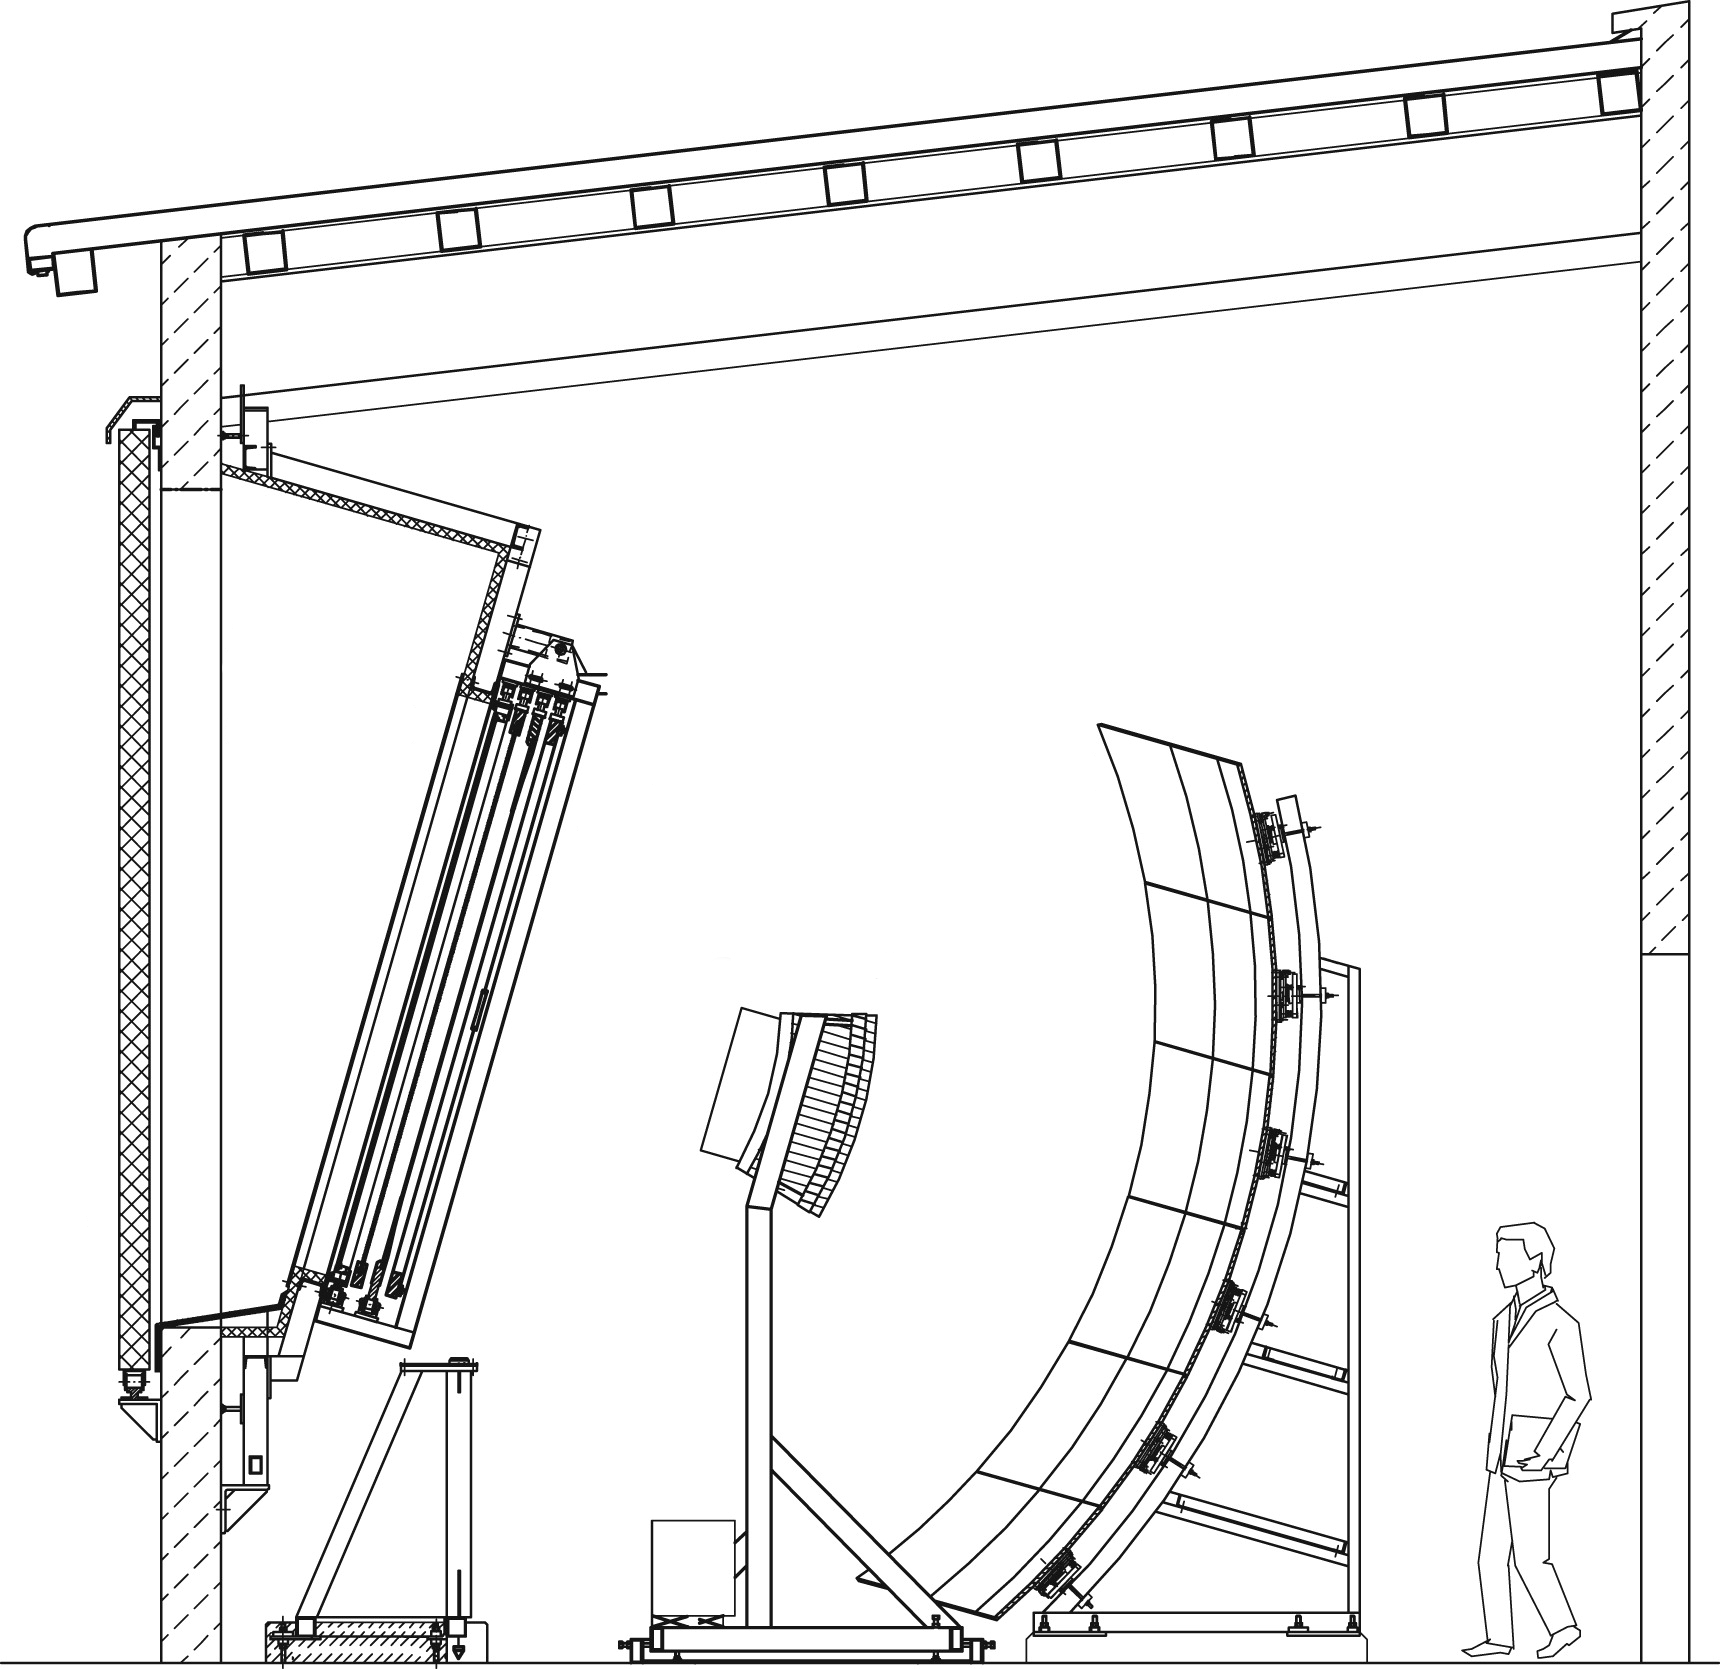
\includegraphics[width=0.48\textwidth]{auger-observatory/fd_schematic.png}
  \label{fig:fd-schematic}
  }
  \caption[]{\subref{fig:auger-map} Overview of the \PAO. The black dots give the 
  location of \WCDs. The blue lines indicate the location and FOV of the \FD. 
  HEAT (red) overlooks the Infill area of the \SD-array. From 
  \cite{veberic_index_nodate}. \subref{fig:fd-schematic} A schematic of a single
  telescope, or bay, of an \FD building, modified from 
\cite{abraham_fluorescence_2010}.}
  \label{fig:pao-images}
\end{figure}


\subsection{Telescope design}
\label{ssec:fd-design}

The \FD telescopes are designed following the schematic of a Schmidt camera with 
corrector plates. The individual components located on the optical axis are, in 
the order that light traverses them:

\begin{itemize}
  \item \textbf{Shutter:} \\
  The shutter consists of two massive metal doors that block the light 
  propagation. Several mechanisms automatically close the shutters to shield the 
  telescope from e.g. atmospheric influences like wind and rain, or an 
  unacceptably high light flux.
  \item \textbf{UV Filter:} \\
  A MUG6 UV-filter is installed in the light path in order to block visible 
  light from entering the telescope, and potentially damaging the sensitive 
  electronics. It separates the climate controlled inside of the \FD buildings 
  from the outside.
  \item \textbf{Corrector:} \\
  A ring of aspheric corrector lenses is located at the edge of the aperture,
  the ring has an inside diameter of \SI{1.7}{\meter} and serves to increase 
  the light collection area, while minimizing spherical aberration in the 
  camera.
  \item \textbf{Curtain:} \\
  The curtain provides a secondary failsafe, that prevents high-intensity light 
  from reaching the electronics. During nominal operation the curtain sits outside 
  of the light path. It can be deployed in emergency situations, or during daytime
  work and maintenance.
  \item \textbf{Mirror:} \\
  The mirrors are a set of hexagonally (square, in the case of \LL) segmented 
  mirrors aligned in a concave $\SI{3.6}{\meter}\times\SI{3.6}{\meter}$ shape, 
  which reflects and concentrates incoming light towards the camera.
  \item \textbf{Camera:} see next subsection.
\end{itemize}

A schematic overview of the setup in each telescope bay is given in
\cref{fig:fd-schematic}.

\subsection{Camera and Readout Electronics}

The camera is made up of 440 highly sensitive \PMTs that make up the individual
pixels. They are arranged in 22 rows and 20 columns. Each pixel has a solid angle 
acceptance of $\Omega = \SI{5.94e-4}{\sr}$. Reflective star shapes with threefold 
symmetry are mounted between pixels. They are commonly referred to as Mercedes 
stars, due to their characteristic shape, and increase both light collection as 
well as ensure a good point resolution between adjacent pixels.

The pixel data is read out at a sampling frequency of \SI{10}{\mega\hertz} 
(\SI{20}{\mega\hertz} in the case of \HE). \todo{continue}


\subsection{High Elevation Auger Telescope (HEAT)}
\label{ssec:heat}

Three additional telescopes, called \HEs are located close to the Coihueco site.
The construction of these telescopes is identical to the telescopes discussed
above. However, in the case of \HE, the entire telescope frame can be rotated,
which allows the observation of the upper atmosphere, and effectively extends the 
energy scale seen by the \FD to lower energies.


\subsection{Telescope Calibration}
\label{ssec:fd-calibration}

The UV-telescopes observe the longitudinal shower profile as an EAS develops. As 
shown in \autoref{chap:cosmic-rays}, this enables the \FD to estimate the total 
energy of the primary particle, by relating it to the count of photons observed 
in the telescope.

The individual pixel PMTs show a drop \todo{is this correct?} in voltage when exposed to UV light. This
voltage gets converted to \ADC via \todo{what?}. The exact \ADC value that a 
given voltage corresponds to is completely determined by the PMT gain, and
fluctuates over the course of a measurement night. Thus in order to obtain a 
physically meaningful observable the conversion factor of \ADC $\rightarrow$ 
photon number needs to be known. This is achieved by illuminating the \FD camera 
with a light source of known intensity, and measuring the camera response. 

\subsubsection{Drum calibration}

The first absolute calibration of the \FD telescopes is the Drum calibration. 


\subsubsection{XY-scanner}



\subsubsection{Calibration A}

In order to track the relative drift between absolute calibration campaigns, an 
LED located in the center of the mirror shoots a known amount of light directly 
at the \FD camera. It is performed twice each night, once before \DAQ, and once 
more after \DAQ.

The importance of this so-called Calibration A becomes apparent when examining the
response of the \FD cameras, as e.g. shown in \autoref{fig:calibration-a-signal}.
Comparing measurements across a larger timespan, it can be seen that the Cal A
before \DAQ systematically has less recovered signal, i.e. measures fewer \ADC
than the post-\DAQ run, while in both runs the cameras are exposed to the same 
amount of light. Moreover, the recovered signal after extended downtimes is lower
than at the end of a measurement period.

This is a consequence of the \PMT electronics being turned off between measurment 
cycles. Each time this occurs, \PMTs first have to warm up again, until full
collection efficiency for incoming photons is reached.

\todo{cal a plot}


\section{The Surface Detector}
\label{sec:sd}

\todo[inline]{roughly mention design, duty cycle}

\section{Central Data Acquisition System (CDAS)}
\label{sec:cdas}



\section{\Offline and Event Reconstruction}
\label{sec:rec}

\begin{figure}[t]
  \centering
  \subfloat[]{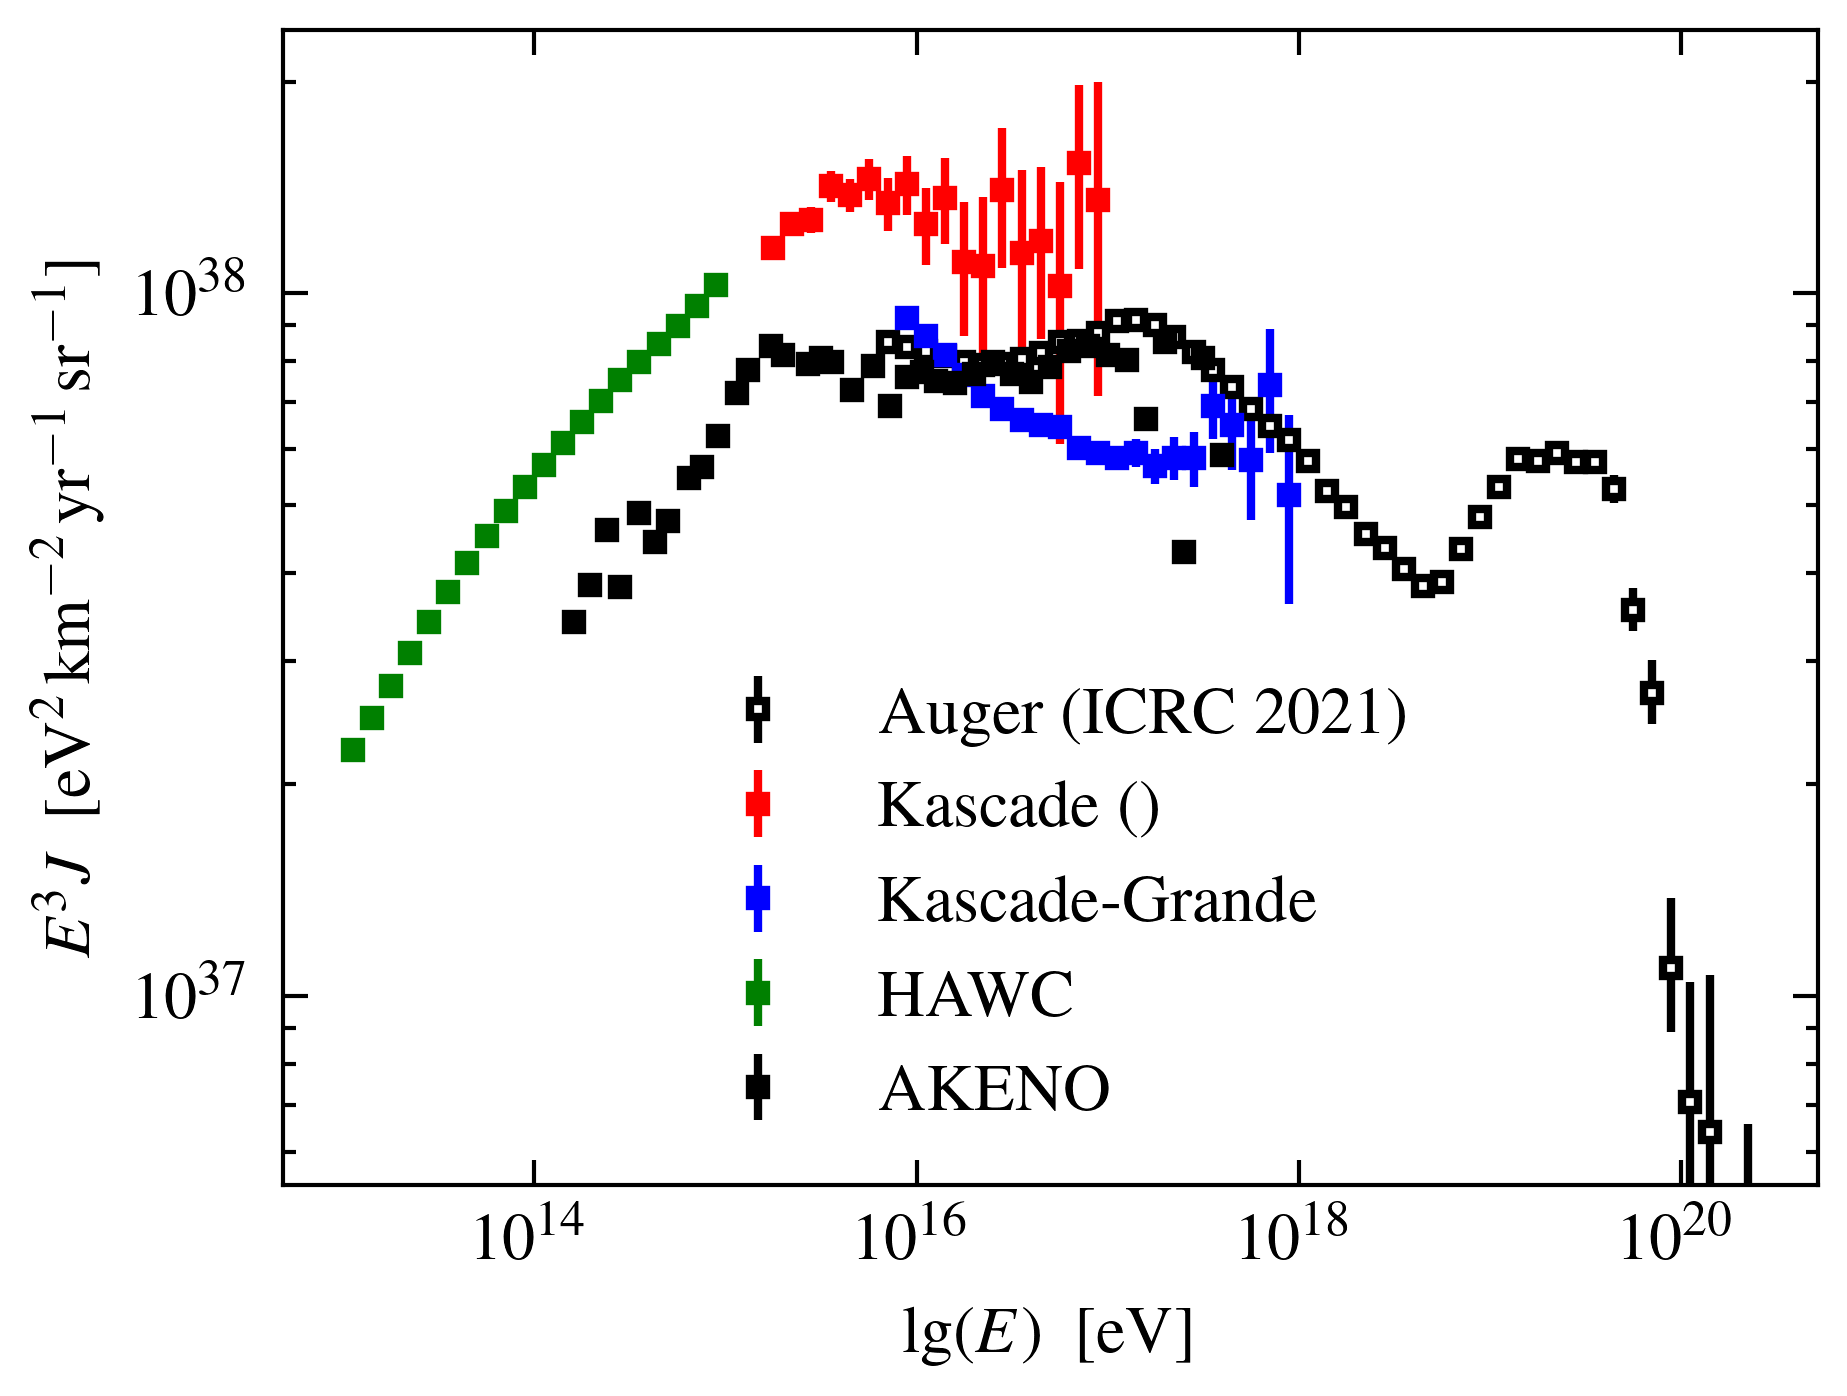
\includegraphics[width=0.47\textwidth]{cosmic-rays/spectrum-double1.png}
  \label{fig:LABEL}
  }\hspace{0.2cm}
  \subfloat[]{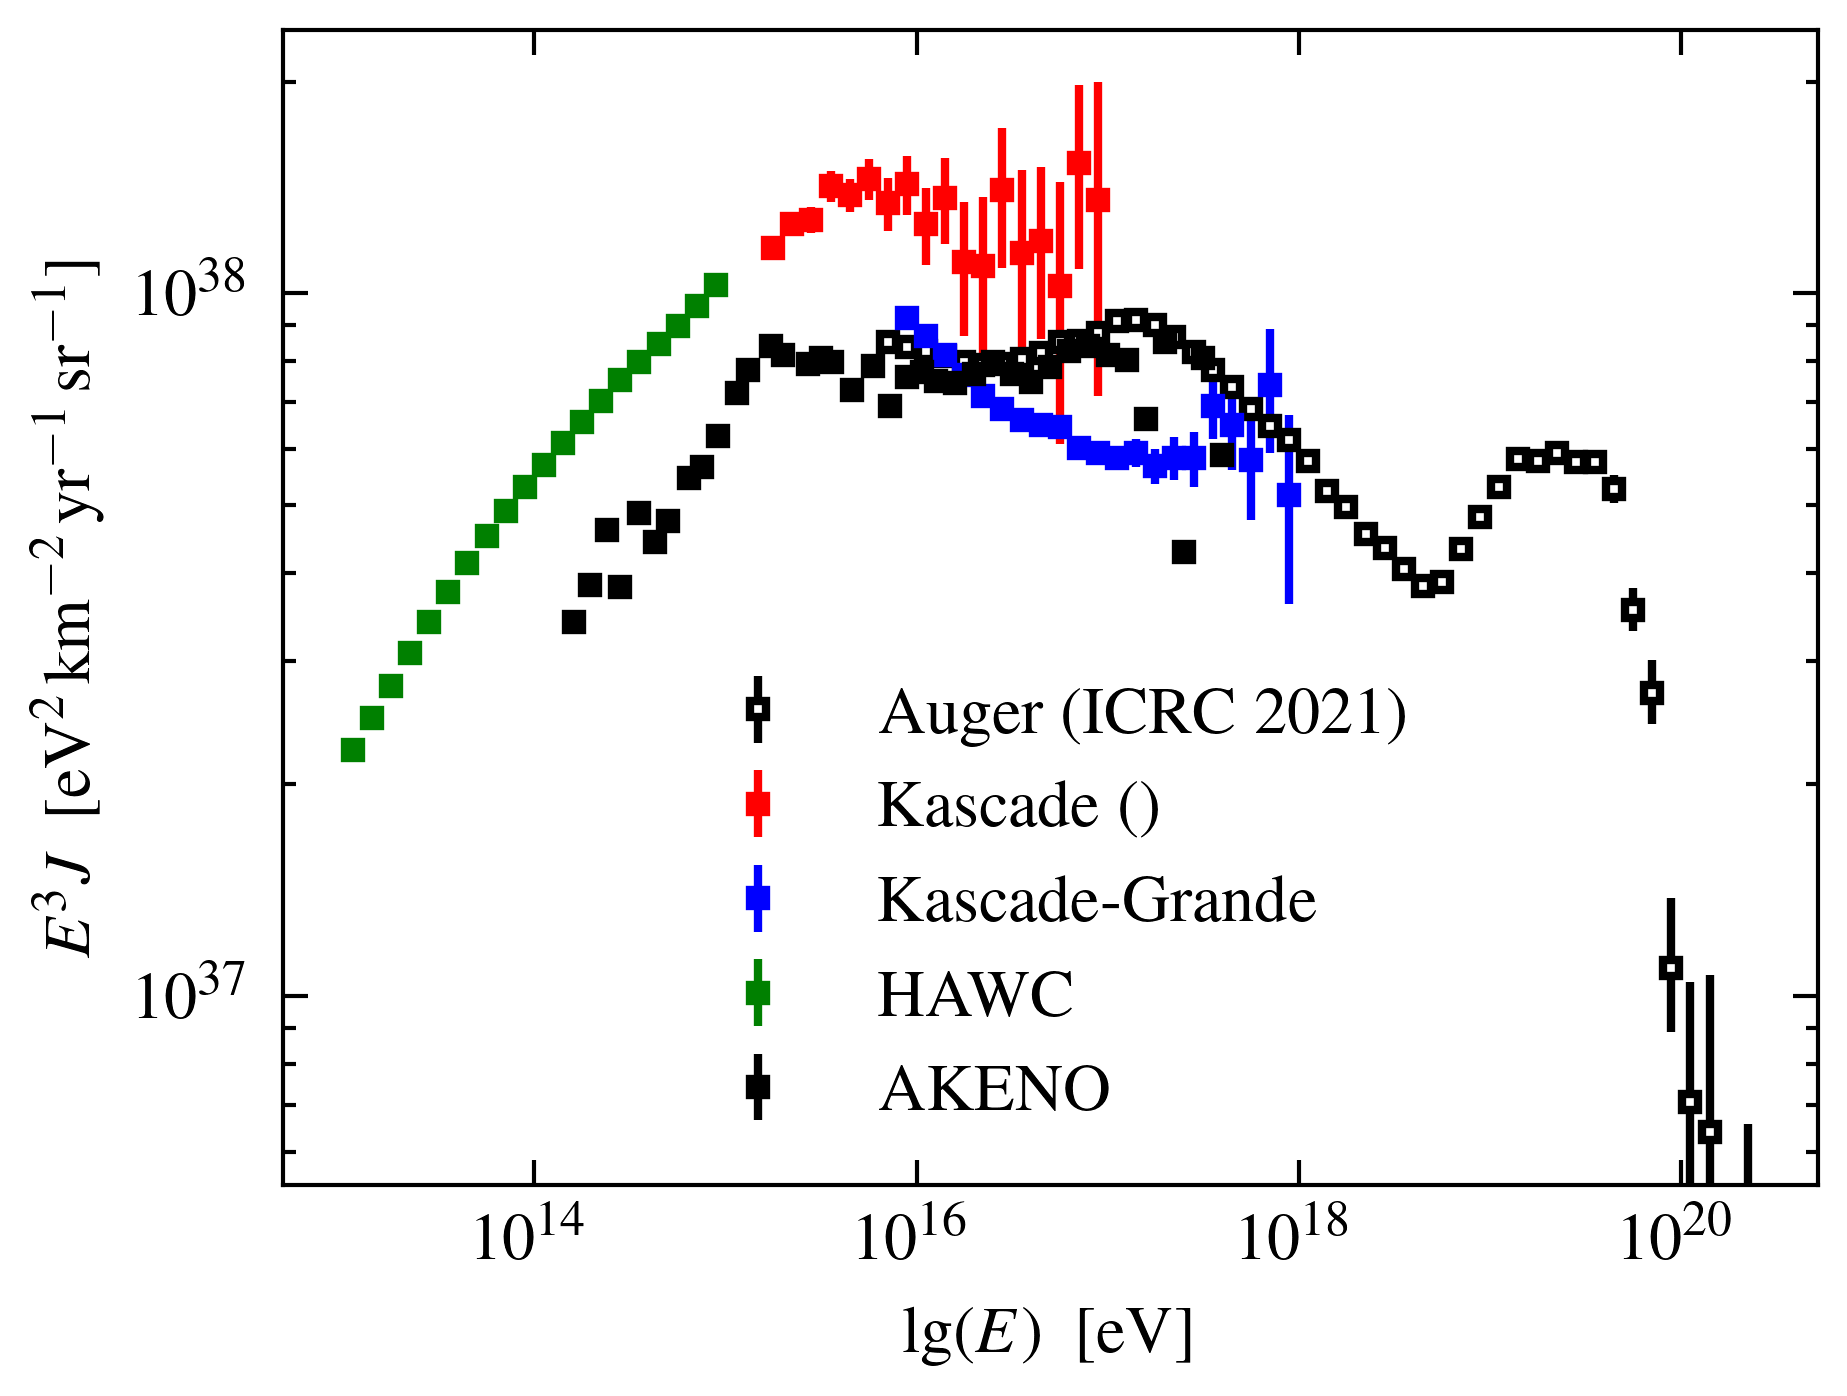
\includegraphics[width=0.47\textwidth]{cosmic-rays/spectrum-double2.png}
  \label{fig:LABEL}
  }
  \caption[]{\subref{fig:LABEL} asdasd \subref{fig:LABEL} asdasd}
  \label{fig:}
\end{figure}

\begin{figure}[t]
  \centering
  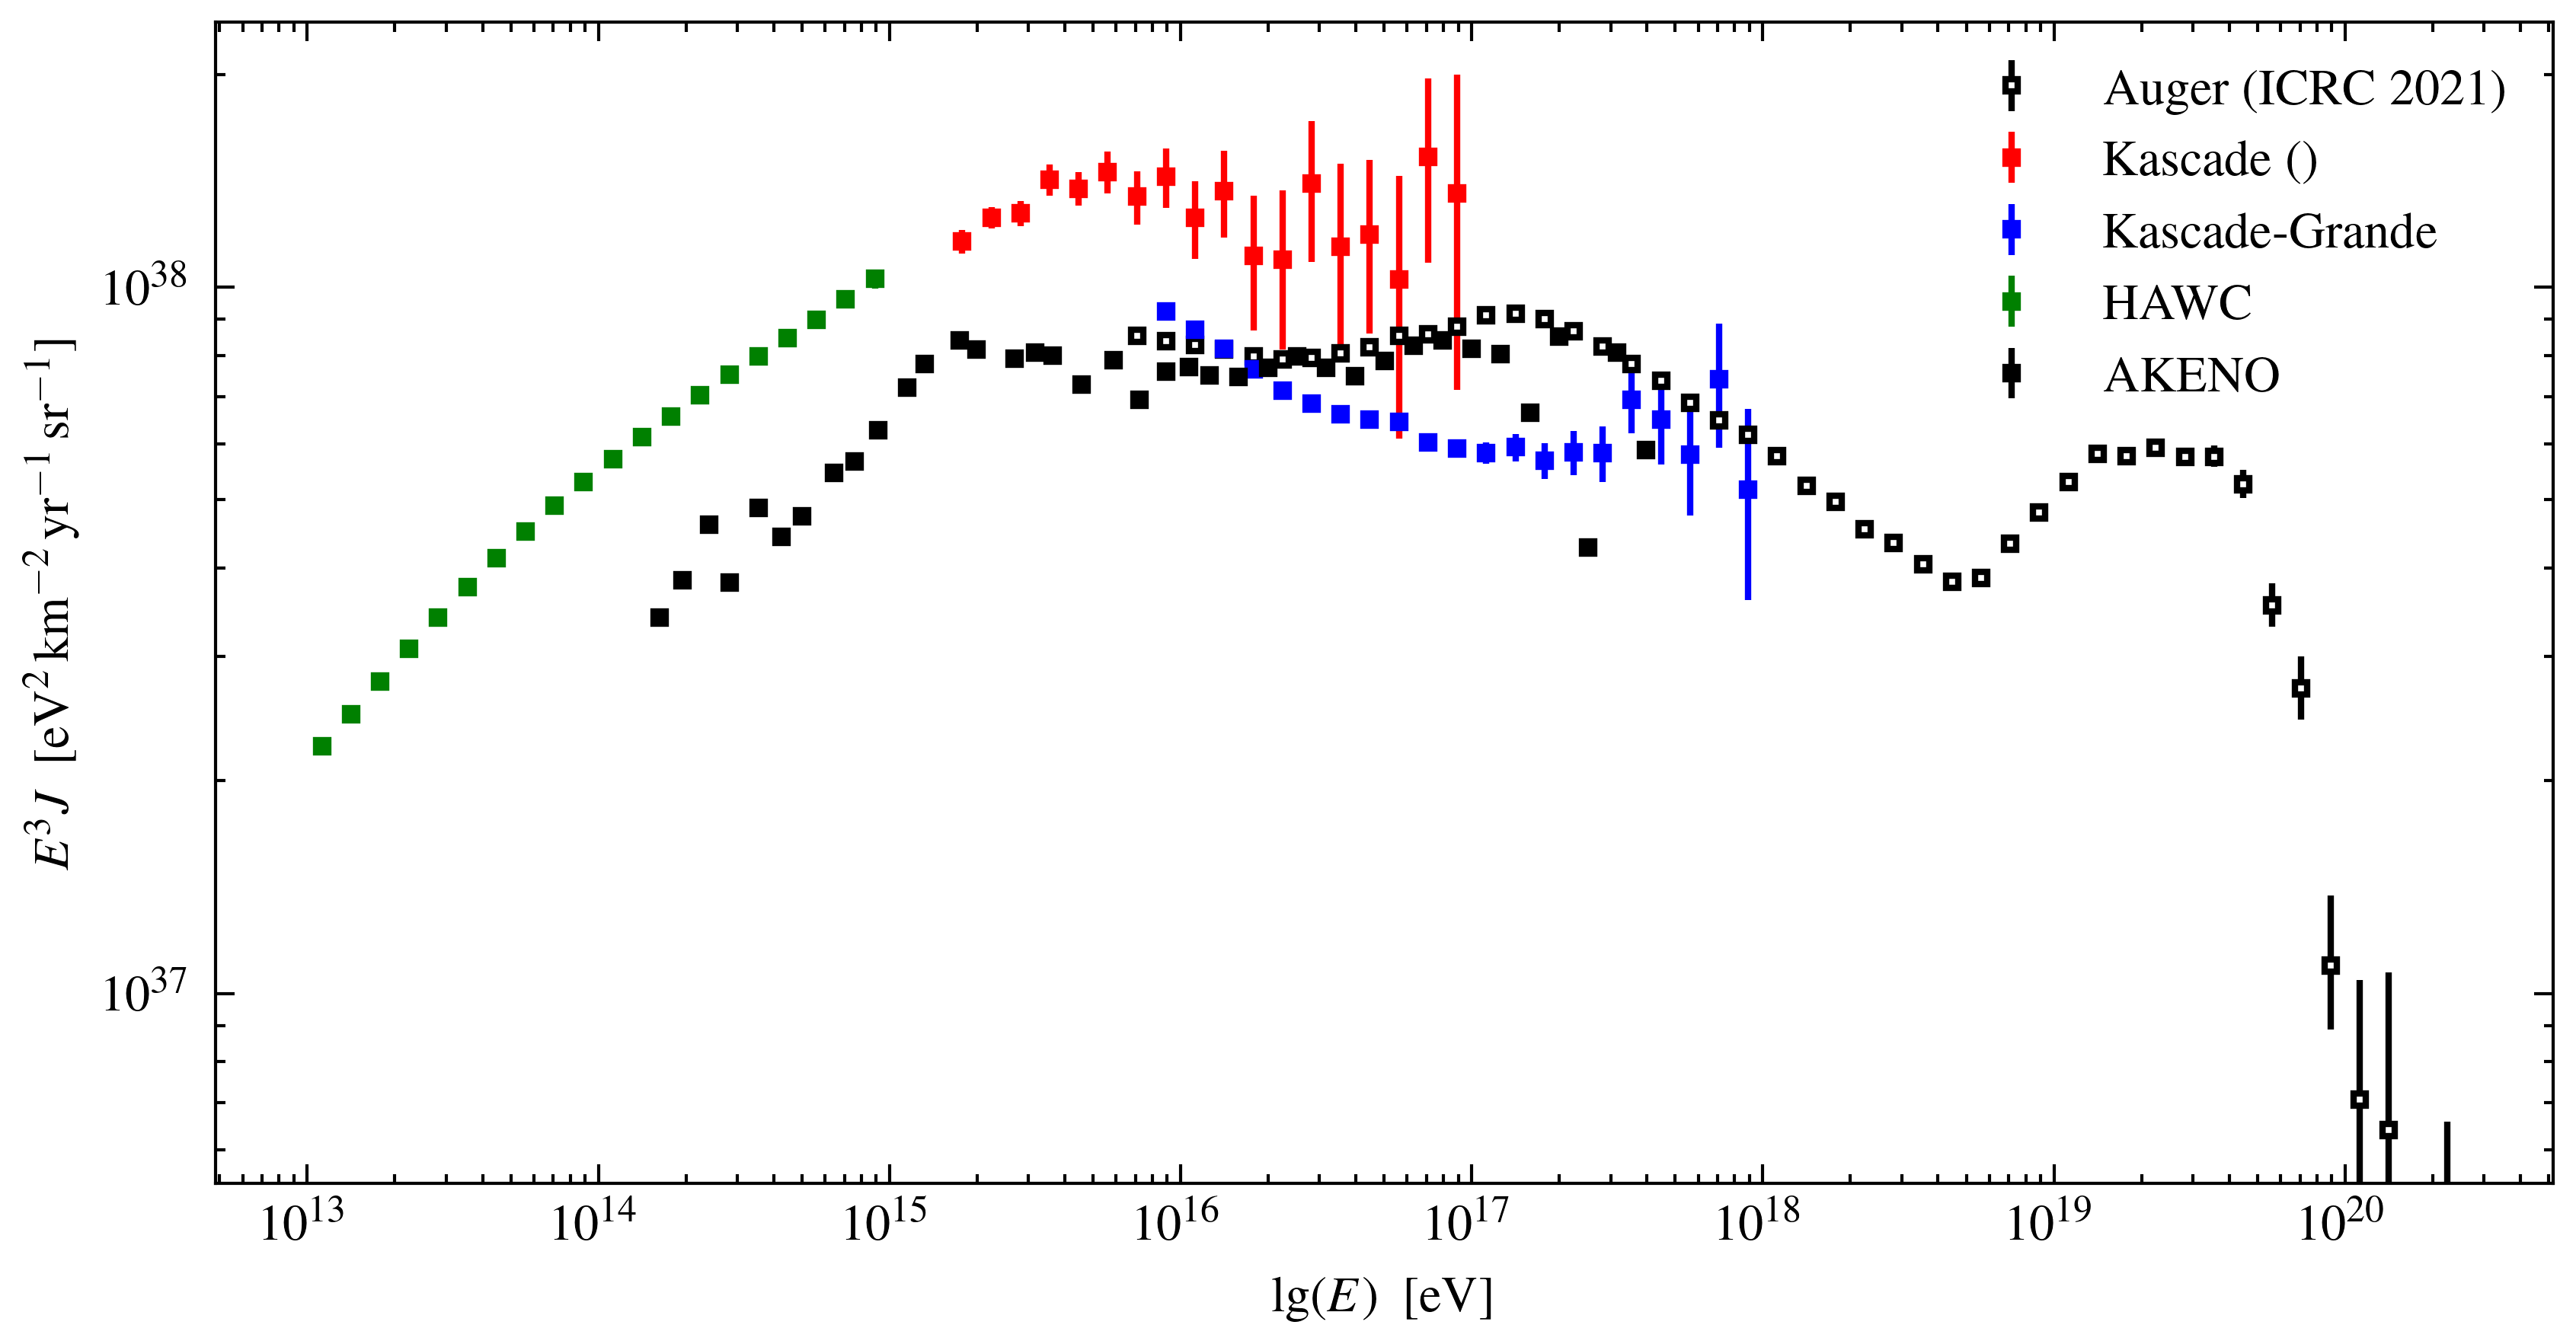
\includegraphics[width=0.9\textwidth]{cosmic-rays/spectrum-single.png}
  \caption{asdasdasdasd}
  \label{fig:asdasd}
\end{figure}

\cref{chap:pierre-auger-observatory} 
